\documentclass{beamer}

\usepackage[utf8]{inputenc}  
\usepackage[frenchb]{babel}
\usepackage[T1]{fontenc}
\usepackage[latin1]{inputenc}
\usepackage{graphicx}
\title{Coût de péages dans le sud de la France}
\author{El Khmissi Mohamed \\ Niasse Gueladio \\ Fontana Quentin }
\date{13 Décembre 2021}

\usetheme{Warsaw}

\begin{document}
% Title page frame
\begin{frame}
    \titlepage 
\end{frame}
% Outline frame
\begin{frame}{Table of contents}
    \tableofcontents
\end{frame}

\AtBeginSection[ ]
{
\begin{frame}{Outline}
    \tableofcontents[currentsection]
\end{frame}
}

% Presentation structure
\section{Le package \texttt{deloqv}}
\subsection{A savoir}
\begin{frame}{A savoir}
\begin{enumerate}
    \item \textbf{Langage de Programmation} : Python
    \item \textbf{Cible} : Reseau autoroutier du Sud de la France (A9, A61, A62, A66, A75 et A709 entre Montpellier, Perpignan, Pamier et Toulouse).
\end{enumerate}
\end{frame}

\subsection{Fonctionnalites}
\begin{frame}{Fonctionnalites}
\begin{enumerate}
    \item \textbf{Produire une Map interactive} : \newline
     \quad - selections des gares de depart et d'arrivee parmis une liste de gares de peage aux choix, \newline
     \quad - visualisation geographique du chemin a parcourir, \newline
     \quad - information sur la distance et sur le cout du trajet. 
    \item Proposer le \textbf{trajet le moins cher} en fonction du nombre d'arrets souhaites en cours de route.
    \item Produire une description de la \textbf{distribution des prix} entre deux gares de peage.
\end{enumerate}
\end{frame}

\section{Etapes de realisation du package \texttt{deloqv}}

\subsection{Preparation des donnees}
\begin{frame}{Traitement puis importation des donnees dans \texttt{VScode}}
\begin{enumerate}
    \item \underline{Creation du dataframe "\texttt{prices.csv}" :} \newline --> conversion et sauvegarde en format \texttt{.csv} des donnees fournies a la page 3 du pdf : \texttt{https://public-content.vinci-autoroutes.com/PDF/\newline Tarifs-peage-asf-vf/ASF-C1-TARIFS-WEB-2021-maille-\newline vf.pdf}
    \item \underline{Creation du dataframe "\texttt{coordonnees.csv}" :} \newline --> Importation du fichier \texttt{gares-peage-2019.csv} disponible a l'url suivant : \texttt{https://www.data.gouv.fr/en/datasets/gares-de-\newline peage-du-reseau-routier-national-concede/}
    \item Transformation du format des coordonnees "X" et "Y" du fichier \texttt{coordonnees.csv} : \newline
    lambert93 (epsg:2154) --> GPS WGS84 (epsg:4326)
\end{enumerate}
\end{frame}

\begin{frame}{Completion et data-cleaning} 
\begin{enumerate}
    \item Suppression des lignes et des colonnes inutiles dans les fichiers \texttt{coordonnees.csv} et \texttt{prices.csv} 
    \item Ajouts des gares de peages et de leurs donnees relatives dans le fichier \texttt{coordonnees.csv}\newline
\newline\newline
\end{enumerate}
Voir code : \texttt{data\underline{ }cleaning.py}
\end{frame}

\subsection{Création de la Map}

\begin{frame}{Création de la Map}

\begin{enumerate}

    \item La partie dataframe: dans cette partie on a utiliser le package \texttt{pandas} pour lire et préparer les bases de données \texttt{coordonnees\underline{}clean.csv} et \texttt{prices\underline{}clean.csv} et une liste contient les noms des 36 villes qu'on a.\newline
    
    \item La partie visualisation : dans cette partie on a utiliser les packages \texttt{folium}, \texttt{openrouteservice} et \texttt{ipywidgets} pour visualiser la map interactive. 


\end{enumerate}

\end{frame}

\begin{frame}{Probléme des distances d'aller-retour}

    \begin{center}
        \begin{tabular}{c c}
                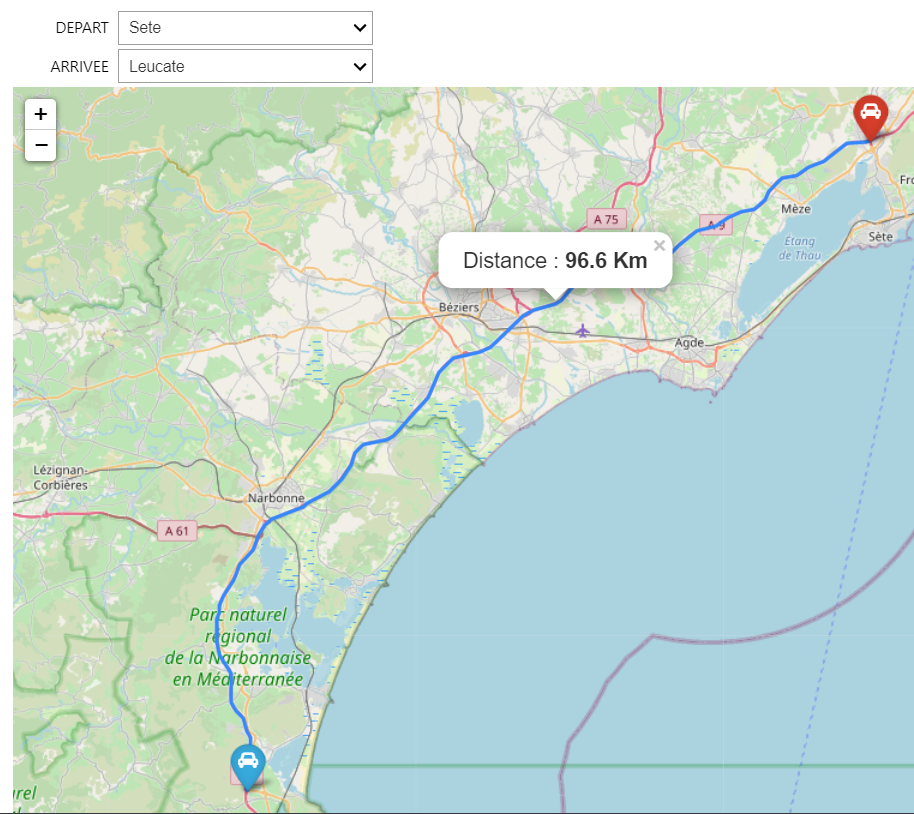
\includegraphics[scale = 0.2]{map prob 1.png} & 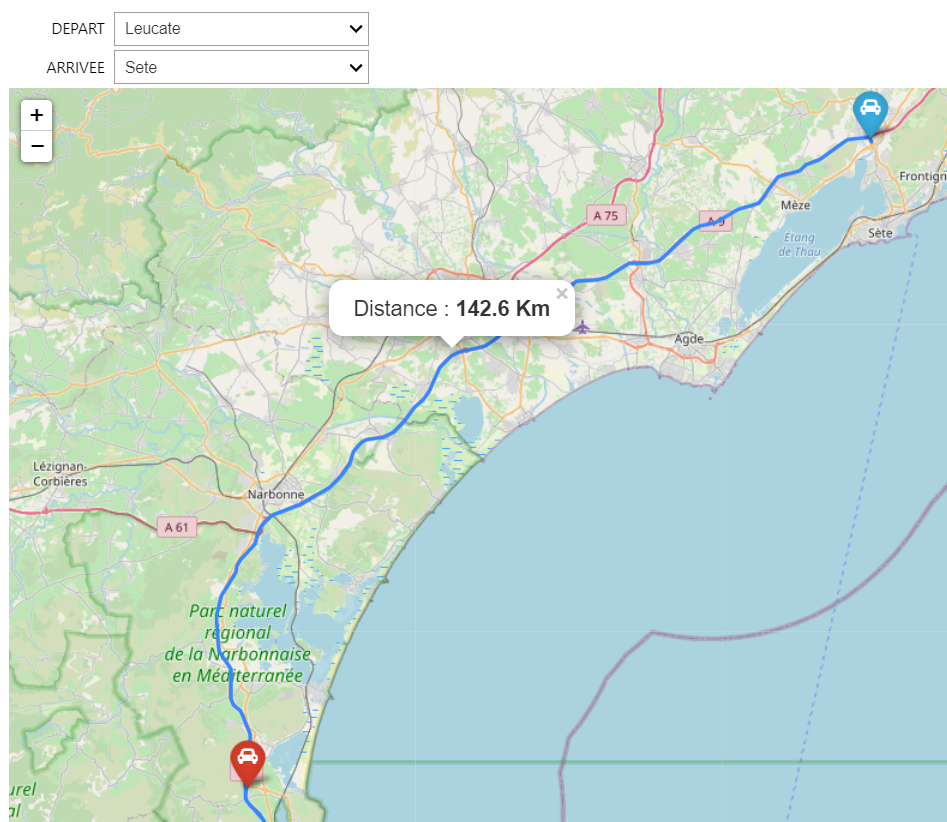
\includegraphics[scale = 0.2]{map prob 2.png} \\
        \end{tabular}
    \end{center}
    
\end{frame}

\begin{frame}{Résolution du probléme des distances}

    \begin{center}
        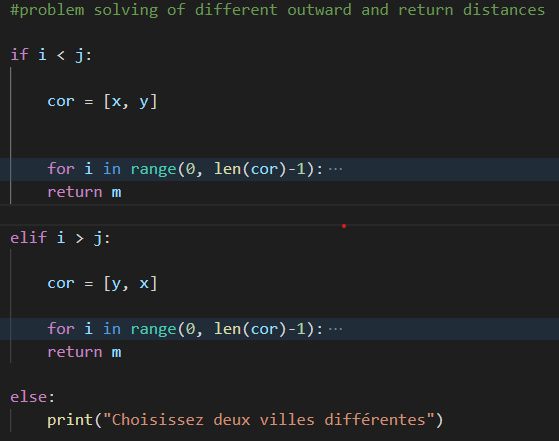
\includegraphics[scale = 0.5]{map solve.png} 
    \end{center}
    
\end{frame}


\begin{frame}{Exemple du visualisation}

    \begin{center}
        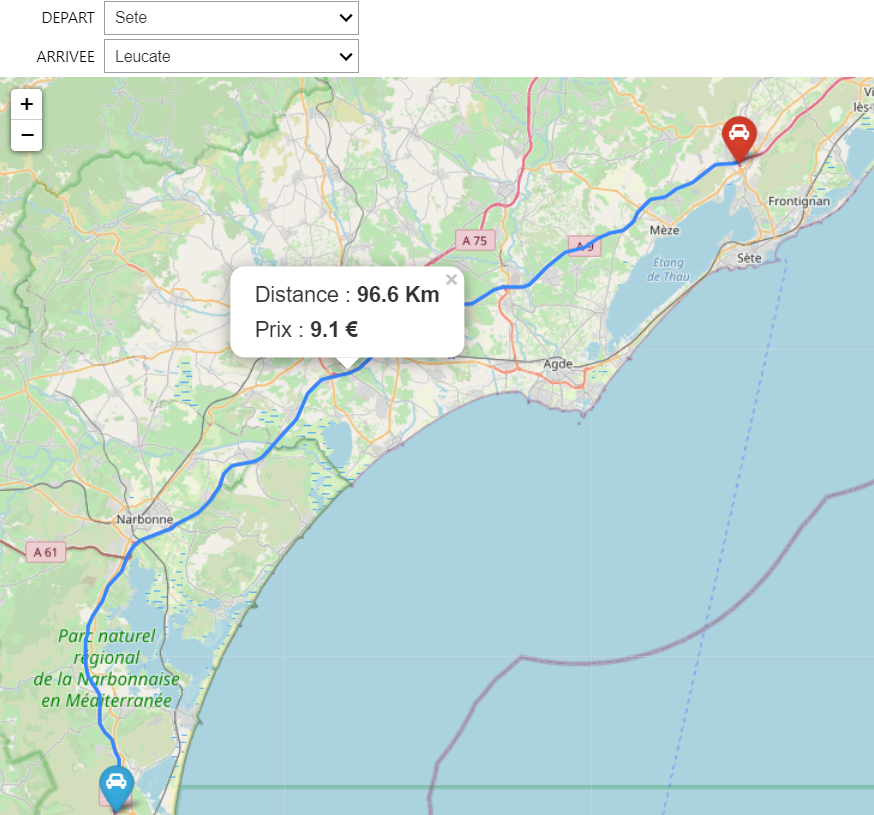
\includegraphics[scale = 0.33]{map.png} 
    \end{center}
    
\end{frame}


\subsection{Algorithme du chemin le moins cher}
\begin{frame}{Problematique}
Comment determiner le trajet a parcourir lorsqu'un voyageur decide de s'arreter \textit{k} fois en cours de route afin que ce trajet lui revienne le moins cher ?
\end{frame}

\begin{frame}{Generation du dataframe d'un trajet correctement indexe} 
\begin{enumerate}
    \item Partitionnement et regroupement des gares de peages
    \item La fonction : \texttt{nb\underline{ }de\underline{ }gare\underline{ }sur\underline{ }trajet(i,j)} : \newline
    --> renvoie le nombre de gares qui separe la gare de depart et d'arrivee.
    \item La fonction composee : \texttt{Le\underline{ }Trajet(tab\underline{ }algo(i,j))} :\newline
    --> renvoie un dataframe ordonne constitue des gares presentes sur le trajet de la gare i a j et dont l'index va de 0 a \texttt{nb\underline{ }de\underline{ }gare\underline{ }sur\underline{ }trajet(i,j)}+1.
\end{enumerate}
\end{frame}

\begin{frame}{Exemple}
    Alfonse est a Perpignan Sud (13) et veut se rendre a Beziers Ouest (7).
    \begin{center}
        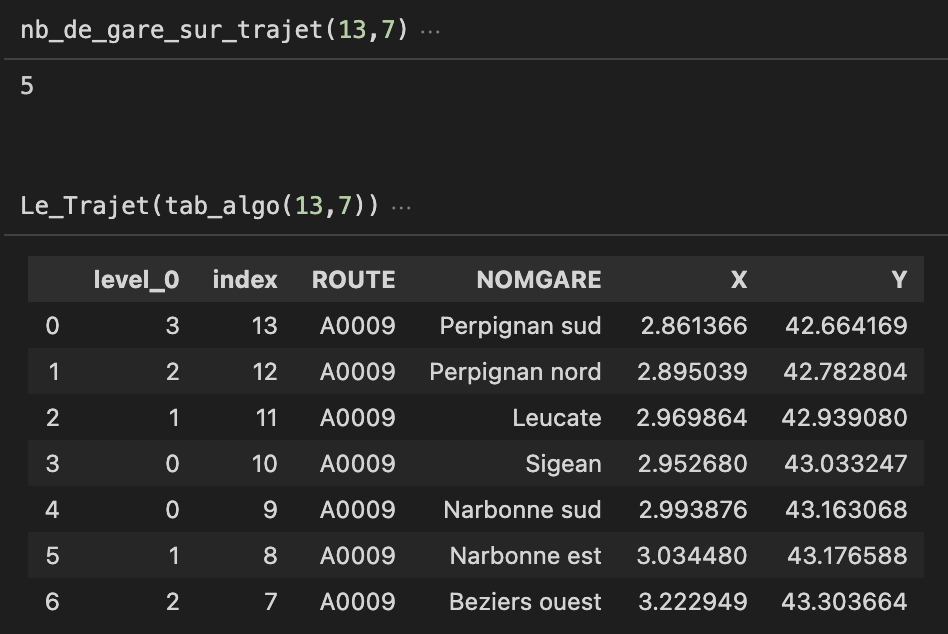
\includegraphics[width=0.8\textwidth]{Algo_1.png}
    \end{center}
\end{frame}
 
 \begin{frame}{Generation de \textit{k}+1 sous-trajets}
 \begin{enumerate}
     \item Fonction \texttt{liste\underline{ }des\underline{ }tuples(p,n)} : \newline
     --> renvoie la liste de tout les arrangements ordonnes possibles de \textit{p} parmis \textit{n} allant de 0 à l'index de la gare d'arrivee. \newline\newline
     \item Fonction \texttt{suite\underline{ }de\underline{ }trajet(p,n)} : \newline
     --> renvoie pour chaque arrangement possible generes par la fonction precedente une suite de couple representant la suite de \textit{k}+1 sous-trajets.
 \end{enumerate}
 \end{frame}
 
 \begin{frame}{Exemple}
    \begin{center}
        \begin{tabular}{c c}
            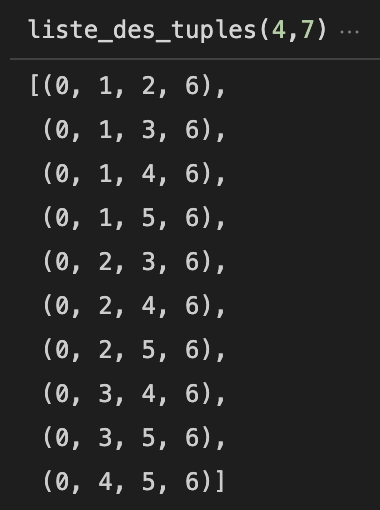
\includegraphics[scale = 0.617]{liste_tuples.png} & 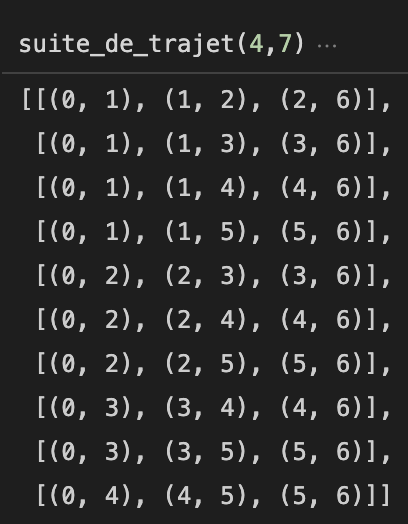
\includegraphics[scale = 0.6]{suite_trajet.png} \\
        \end{tabular}
    \end{center}
\end{frame}
 
 \begin{frame}{Chemin le moins cher}
 \begin{itemize}
     \item Fonction \texttt{cout\underline{ }minimum(data,depart,arrivee)} : \newline
     - arguments :
     \begin{itemize}
         \item data = \texttt{Le\underline{ }Trajet(tab\underline{ }algo(i,j))}
         \item depart = 0
         \item arrivee = \texttt{nb\underline{ }de\underline{ }gare\underline{ }sur\underline{ }trajet(i,j)}+1
     \end{itemize}
     --> renvoie le cout d'un trajet lorsqu'il se fait sans arret.
 \end{itemize}
 \end{frame}
 
 \begin{frame}{Chemin le moins cher}
 \begin{itemize}
 \item Fonction \texttt{cout\underline{ }minimum\underline{ }tuple(depart,arrivee,k,data)} : \newline
     - arguments :
     \begin{itemize}
         \item data = \texttt{Le\underline{ }Trajet(tab\underline{ }algo(i,j))}
         \item depart = 0
         \item arrivee = \texttt{nb\underline{ }de\underline{ }gare\underline{ }sur\underline{ }trajet(i,j)}+1
         \item k = nombre d'arrets
     \end{itemize}
     --> renvoie le cout minimum d'un trajet en fonction de \textit{k}.
 \end{itemize}
 \end{frame}
 
\begin{frame}{Exemple}
Alfonse decide de s'arreter deux fois en cours de route. Il voudrait savoir a quelle gare de peage sortir afin que le cout de son trajet soit minimise. Il utilise donc notre algorithme. \begin{center}
    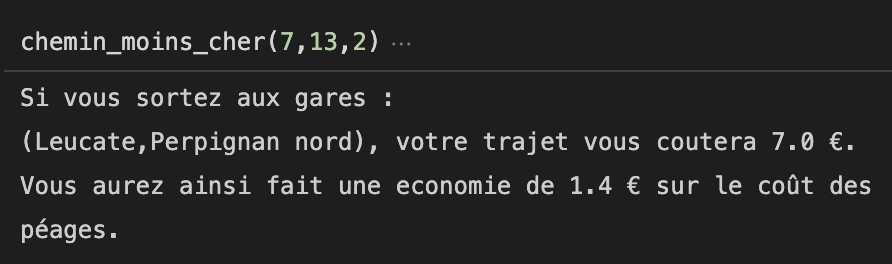
\includegraphics[scale = 0.7]{cheminmoinscher.png}
\end{center}
\end{frame} 
 
 \subsection{Distribution des prix}
 \begin{frame}{Objectif}
     Determiner la distribution des prix des peages par kilometre suivant un trajet donne.
 \end{frame}
 
 \begin{frame}{Principe}
     \begin{enumerate}
     \item Choisir un trajet a etudier
         \item Rechercher dans le dataframe des prix la donnee relative au cout de peage entre chaque gares successives presentes sur le trajet.
         \item Diviser respectivement chacun des prix retenus par la distance en kilometres qui separe les gares.
         \item Rapprocher tout les resultats sous la forme d'une courbe de densitee dans un plot a l'aide de la fonction \texttt{kdeplot} fournie par le package \texttt{seaborn}.
     \end{enumerate}
 \end{frame}
 
 \begin{frame}{Exemple}
     \begin{center}
         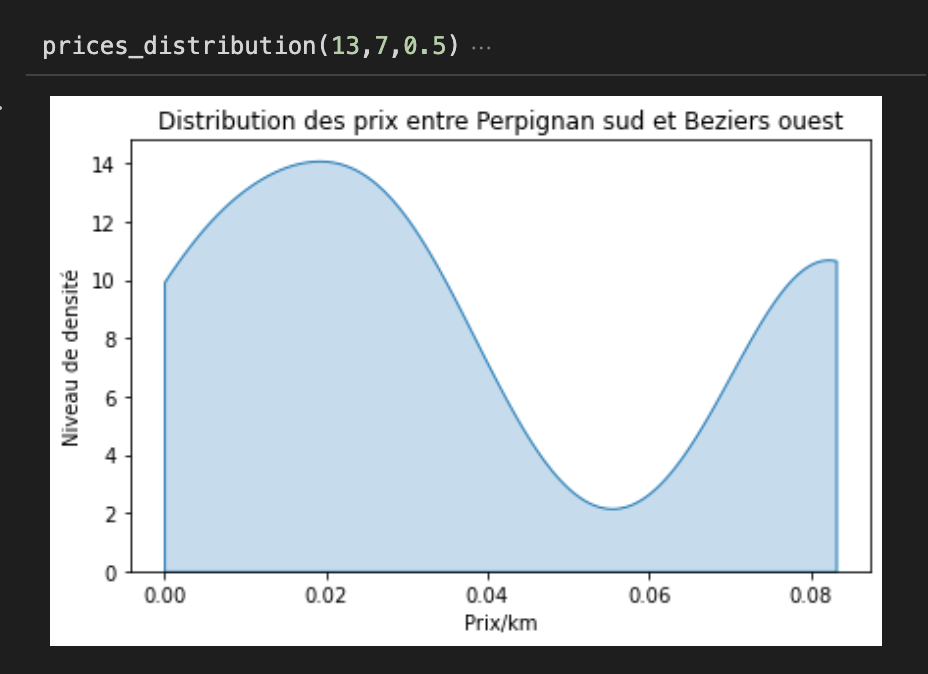
\includegraphics[scale = 0.6]{prices_distrib.png}
     \end{center}
 \end{frame}


\section{Presentaion de la Doc}

    \subsection{Problem}
\begin{frame}
$-$ Objectif du project
\end{frame}
    \subsection{Install}
         \subsubsection{Aspect github}
           \subsubsection{Packages utlies}
 \begin{frame}
 $-$ Pandas \\
 $-$ Folium \\
 $-$ osmix \\
 $-$ networkx\\
 
 
\end{frame}

    \subsection{Contact and Sources}

\section{Synthese}



\end{document}
